\newcommand{\pluseq}{\mathrel{+}=}

\subsection{Recap: Quality Assurance}

\begin{frame}{\myframetitle\ \mytitlesource{\ludewiglichter}}
	\hfill%
	\only<1|handout:0>{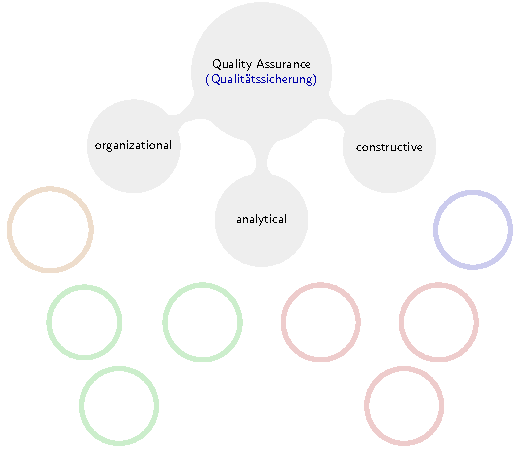
\includegraphics[height=\textheightwithtitle,page=1]{quality-assurance}}%
	\only<2|handout:0>{\includegraphics[height=\textheightwithtitle,page=2]{quality-assurance}}%
	\only<3|handout:0>{\includegraphics[height=\textheightwithtitle,page=3]{quality-assurance}}%
	\only<4|handout:0>{\includegraphics[height=\textheightwithtitle,page=4]{quality-assurance}}%
	\only<5|handout:1>{\includegraphics[height=\textheightwithtitle,page=5]{quality-assurance}}%
	\only<6|handout:0>{\includegraphics[height=\textheightwithtitle,page=6]{quality-assurance}}%
\end{frame}

%mit nem emotionalen Bild/bsp motivieren => gute Softwarequalität ist wichtig

\subsection{Automated Analysis of Product Lines}

\begin{frame}{\myframetitle}
	% \begin{mycolumns}
	% 	\mynote{Open Questions}{
	% 		\begin{itemize}
	% 			\item How do such configurators work?
	% 			\item How to avoid inconsistencies?
	% 			\item How to provide explanations and fixes?
    % 			\item How to get all valid configurations automatically? (\emph{P2(b)})
	% 		\end{itemize}
	% 	}
	% 	\mydefinition{Automated Analysis of Feature Models}{
	% 		\begin{itemize}
	% 			\item up until now: \emph{creation} and \emph{transformation} of feature models
	% 			\item now: \emph{analysis} of feature models to improve our understanding of a configuration space
	% 			\item for brevity: product = valid configuration
	% 		\end{itemize}
	% 	}
	% \mynextcolumn
	% 	\myexample{Asking Questions About Product Lines}{
	% 		(in ascending order of difficulty)
	% 		\begin{itemize}
	% 			\item Can we test 
	% 			\item Can we compile every product successfully?
	% 			\item Can we test every product successfully?
	% 			\item 
	% 			\item Is a given configuration valid?
	% 			\item Is there any product at all?\\
	% 				How many/which products are there?\\
	% 			\item Is a given feature (de-)selectable at all?\\
	% 				How many/which products include it?\\
	% 			\item Is a given partial configuration consistent?\\
	% 				How many/which products include it?\\
	% 			\item \color{gray}{(Which features always occur together?)}
	% 			\item \color{gray}{(Is a given constraint redundant?)}
	% 			\item \color{gray}{(How do two feature model versions differ?)}
	% 			\item \color{gray}{(Why is \ldots? How to fix \ldots?)}
	% 		\end{itemize}
	% 	}
	% \end{mycolumns}
\end{frame}

\subsection{Product-Based Analysis Strategy}

\begin{frame}{\myframetitle}
	\begin{mycolumns}
		\mydefinition{Intuition}{
			\begin{itemize}
				\item to analyze the product line, just analyze \emph{each product}
				\begin{itemize}
					\item individually
					\item in isolation
					\item possibly in parallel
				\end{itemize}
			\end{itemize}
		}
		\myexampletight{}{\centering\featureDiagramLego}
	\mynextcolumn
		\pic[width=\linewidth,page=9]{lego-analyses}
	\end{mycolumns}
\end{frame}

\begin{frame}{\myframetitle}
	\begin{mycolumns}
		\mydefinition{Generic Algorithm}{
			\begin{algorithmic}
				\Require a product line with a feature model $FM$
				\Ensure runs a given analysis $\alpha$ on all products
				\State $C \gets AllSAT(\phi(FM))$ \Comment{{\small enumerate valid config's}}
				\State $results \gets []$
				\ForAll{$S \in C$} \Comment{{\small for each valid config}}
				\State $P \gets \gamma(S)$ \Comment{{\small generate the product}}
				\State $results \pluseq \alpha(P)$ \Comment{{\small append the analysis result}}
				\EndFor
				\State \Return $\sigma(results)$
			\end{algorithmic}
		}
		\mynote{}{
			\begin{itemize}
				\item $\gamma$ \emph{generates} (= compiles) products (e.g., \texttt{make}, \texttt{gradle}, \texttt{FeatureHouse}, \texttt{npm}, \ldots)
				\item $\alpha$ \emph{analyzes} the product (e.g., run all tests)
				\item $\sigma$ \emph{summarizes} the results (e.g., each individual call to $\alpha$ must succeed)
			\end{itemize}
		}
	\mynextcolumn
		\myexampletight{}{
			\begin{center}
				\small\featureDiagramConfigurableDatabase
			\end{center}
		}
		\myexample{}{
			\footnotesize
			\leftandright{
				$\sigma([\alpha(\gamma(\{C,G,W\}))$\\
				$~~~~\alpha(\gamma(\{C,P,W\})$\\
				$~~~~\alpha(\gamma(\{C,G,P,W\}))$\\
				$~~~~\alpha(\gamma(\{C,D,W\}))$\\
				$~~~~\alpha(\gamma(\{C,G,D,W\}))$\\
				$~~~~\alpha(\gamma(\{C,P,D,W\}))$\\
				$~~~~\alpha(\gamma(\{C,G,P,D,W\}))$\\
				$~~~~\alpha(\gamma(\{C,P,T,W\}))$\\
				$~~~~\alpha(\gamma(\{C,G,P,T,W\}))$\\
				$~~~~\alpha(\gamma(\{C,D,T,W\}))$\\
				$~~~~\alpha(\gamma(\{C,G,D,T,W\}))$\\
				$~~~~\alpha(\gamma(\{C,P,D,T,W\}))$\\
				$~~~~\alpha(\gamma(\{C,G,P,D,T,W\}))$
			}{
				$\alpha(\gamma(\{C,G,L\}))$\\
				$\alpha(\gamma(\{C,P,L\}))$\\
				$\alpha(\gamma(\{C,G,P,L\}))$\\
				$\alpha(\gamma(\{C,D,L\}))$\\
				$\alpha(\gamma(\{C,G,D,L\}))$\\
				$\alpha(\gamma(\{C,P,D,L\}))$\\
				$\alpha(\gamma(\{C,G,P,D,L\}))$\\
				$\alpha(\gamma(\{C,P,T,L\}))$\\
				$\alpha(\gamma(\{C,G,P,T,L\}))$\\
				$\alpha(\gamma(\{C,D,T,L\}))$\\
				$\alpha(\gamma(\{C,G,D,T,L\}))$\\
				$\alpha(\gamma(\{C,P,D,T,L\}))$\\
				$\alpha(\gamma(\{C,G,P,D,T,L\}))])$
			}
		}
	\end{mycolumns}
\end{frame}

\begin{frame}[fragile]{\myframetitle}
	\begin{mycolumns}[columns=3,widths={25,50,25}]
	\mynextcolumn
		\hspace*{-6mm}\href{https://dl.acm.org/doi/abs/10.1145/3382025.3414943}{\includegraphics[width=1.2\linewidth,trim=180 510 100 170,clip]{2020/2020-SPLC-Thuem}}
		\mynote{Advantages and Challenges}{
			\begin{itemize}
				\item[+] sound and complete (if generator $\gamma$, analysis $\alpha$, and summary $\sigma$ are sound and complete)
				\item[--] does not scale to realistic product lines
				\begin{itemize}
					\item $AllSAT$ only works on small feature models
					\item up to $2^{\abs{F}}$ calls to the generator $\gamma$ and the analysis $\alpha$
				\end{itemize}
			\end{itemize}
		}
	\mynextcolumn
	\end{mycolumns}
\end{frame}

% \subsection{Sample-Based Testing} % maybe move to lec 11 with recap of product-based

% \begin{frame}{\myframetitle}
% 	\begin{mycolumns}
% 		\mydefinition{Intuition}{
% 			\begin{itemize}
% 				\item to analyze the product line, just analyze \emph{some products} (which products?)
% 				\item e.g., \emph{sample-based testing} \lecturetesting
% 			\end{itemize}
% 		}
% 		\mynote{Advantages and Challenges}{
% 			\todots
% 		}
% 	\mynextcolumn
% 		\pic[width=\linewidth,page=10]{lego-analyses}
% 	\end{mycolumns}
% \end{frame}

\subsection{Feature-Based Analysis Strategy}

\begin{frame}{\myframetitle}
	\begin{mycolumns}
		\mydefinition{Intuition}{
			\begin{itemize}
				\item to analyze the product line, just analyze \emph{some products} (which products?)
				\item e.g., \emph{sample-based testing} \lecturetesting
			\end{itemize}
		}
		\mynote{Advantages and Challenges}{
			\todots
		}
	\mynextcolumn
		\pic[width=\linewidth,page=6]{lego-analyses}
	\end{mycolumns}
\end{frame}

\subsection{Family-Based Analysis Strategy}

\begin{frame}{\myframetitle}
	\begin{mycolumns}
		\mydefinition{Intuition}{
			\begin{itemize}
				\item to analyze the product line, just analyze \emph{some products} (which products?)
				\item e.g., \emph{sample-based testing} \lecturetesting
			\end{itemize}
		}
		\mynote{Advantages and Challenges}{
			\todots
		}
	\mynextcolumn
		\pic[width=\linewidth,page=3]{lego-analyses}
	\end{mycolumns}
\end{frame}

\subsection{Classification of Product-Line Analysis Strategies}

\begin{frame}{\myframetitle}
	\begin{mycolumns}[columns=3]
		\pic[width=\linewidth,page=9]{lego-analyses}

		\mydefinition{Product-Based Strategy}{
			\begin{itemize}
				\item[+] sound and complete %(if generator $\gamma$, analysis $\alpha$, and summary $\sigma$ are sound and complete)
				\item[--] does not scale in general %to realistic product lines
				\begin{itemize}
					\item $AllSAT$ only works on small feature models
					\item up to $2^{\abs{F}}$ calls to the generator $\gamma$ and the analysis $\alpha$
				\end{itemize}
			\end{itemize}
		}
	\mynextcolumn
		\pic[width=\linewidth,page=6]{lego-analyses}
	
		\mydefinition{Feature-Based Strategy}{
			\todots
		}
	\mynextcolumn
		\pic[width=\linewidth,page=3]{lego-analyses}

		\mydefinition{Family-Based Strategy}{
			\todots
		}
\end{mycolumns}
\end{frame}

% mit quadranten starten
%bezug auf FM-analyse
%wir gucken uns jetzt Source Code an (evtl. linke zwei (VL 4, Problem Space) + rechte zwei Quadranten (VL 10+, Solution Space))
% wechselwirkung zw. sol und problem space (mapping+FM)

% properties one might want to analyze, similar to questions about feature models in modeling.tex
% include questions for all four quadrants

%strategien high-level angucken
%product-based
%number crunching, wie groß sind SPLs, product-based skaliert nicht

%ich könnte weniger produkte angucken (sampling)
%grundstein für test-vorlesung

%oder nur features angucken: feature-based
%wichtige message: es reicht nicht, features einzeln zu analysieren
%rückgriff auf interaktionen (dass feature-based nicht reicht)

\subsection{Complexity of Product-Line Analyses}

\begin{frame}{\myframetitle}
	\leftorright{
		\mydefinition{Six Classes of Product-Line Complexity \mytitlesource{\href{https://youtu.be/qUuRp7_d0rU?t=1651}{Thüm~2021}}}{
			In a timeframe of 24h \ldots
			\begin{enumerate}
				\item[\color{gray}\textbf{NC}] {\color{gray}Products cannot be generated automatically}
				\item[\textbf{C1}] All products can be generated and \emph{tested}
				\item[\textbf{C2}] Not C1, but all \emph{products} can be \emph{generated}
				\item[\textbf{C3}] Not C2, but all \emph{configurations} can be \emph{generated} (AllSAT)
				\item[\textbf{C4}] Not C3, but the \emph{number of valid configurations} can be computed (\ssat{})
				\item[\textbf{C5}] Not C4, but \emph{whether there is a valid configuration} can be computed (SAT)
				\item[\textbf{C6}] It cannot be computed whether there is a valid configuration
			\end{enumerate}
		}
	}{
		\myexample{Examples}{
			\begin{enumerate}
				\item[\color{gray}\textbf{NC}] {\color{gray}all product lines with custom development in application engineering\\(e.g., components and services with glue code, white-box frameworks)}
				\item[\textbf{C1}] $< 2000$ products for 1 min per product
				\item[\textbf{C2}] $< 90000$ products for 1 s per product
				\item[\textbf{C3}] $< 10^{13}$ configurations for 1 ns per configuration
				\item[\textbf{C4}] older versions of Linux/Automotive05
				\item[\textbf{C5}] newer versions of Linux/Automotive05\\(see \evaluatingsharpsatsolvers)
				\item[\textbf{C6}] No example known
			\end{enumerate}
		}
	}
\end{frame}